\documentclass[conference]{IEEEtran}
\usepackage{amsmath,amsfonts,graphicx}
\usepackage{listings}
\usepackage{xcolor}
\usepackage{caption}
\usepackage{booktabs}
\usepackage{float}

\definecolor{codegray}{gray}{0.95}
\lstset{
  backgroundcolor=\color{codegray},
  basicstyle=\ttfamily\footnotesize,
  breaklines=true,
  frame=single,
  postbreak=\mbox{\textcolor{red}{$\hookrightarrow$}\space},
  keywordstyle=\color{blue},
  commentstyle=\color{gray},
  stringstyle=\color{orange},
  language=Python
}

\setlength{\columnsep}{25pt}

\title{Convolutional Neural Network: An Educational Perspective Through a Pure Python Implementation}

\author{
  \IEEEauthorblockN{Bui Tuan Minh}
  \IEEEauthorblockA{
    \textit{Department of Information and Communication Technology} \\
    \textit{University of Science and Technology of Hanoi} \\
    Email: minhbt2440041@usth.edu.vn}
}

\raggedbottom

\begin{document}

\maketitle

\begin{abstract}
In this project, I created a minimal yet instructive implementation of a Convolutional Neural Network (CNN) from scratch using only Python's \texttt{math} and \texttt{matplotlib} libraries. This implementation showcases the underlying mechanisms of CNNs, such as convolution, activation functions, flattening, pooling, and fully connected layers. The goal is to attain a deeper understanding of the fundamentals of deep learning.
\end{abstract}

\section{Introduction}
Convolutional Neural Networks (CNNs) play a key role in modern machine learning, especially in computer vision tasks. Their layered structure allows them to detect patterns in images in a step-by-step way, starting from simple edges and building up to more complex shapes. However, the widespread use of high-level libraries like TensorFlow and PyTorch often hides the details of how CNNs actually work.

This project takes a different approach by building a CNN manually without relying on those high-level tools. Doing so gives a clearer view of how data moves through the network, how tensors are transformed at each stage, and how the learning process unfolds. This makes the method especially useful for educational purposes.

Although modern frameworks offer powerful tools, they can sometimes make it harder for beginners to truly understand what’s happening under the hood. By constructing a CNN from scratch, learners get to see how each convolutional layer, activation, pooling, and dense contribute to how the model learns. This hands-on approach helps break down the "black box" reputation of deep learning and shows why each step matters for recognizing features and making predictions.

Building a CNN manually also deepens understanding of important topics like optimization, loss functions, and the practical challenges of training neural networks. It brings attention to the trade-offs involved, such as speed and scalability when working at a low level. Through this project, my goal is to bridge the gap between theory and practice, helping students and practitioners develop a stronger, more intuitive grasp of how deep learning really works.

\section{Architecture Overview}
My implementation consists of:
\paragraph{Convolutional Layer:} The first part of my network is a single convolutional layer. It uses a small filter that moves across the image, looking at small sections and calculating patterns by multiplying and summing pixel values. This creates a feature map that captures simple details like edges or textures. By using just one filter, the setup stays simple and easy to understand, making it clearer how the model starts to pick up useful features from the raw image.

\paragraph{ReLU Activation:} After convolution, the feature map is passed through a Rectified Linear Unit (ReLU) activation function. ReLU introduces non-linearity by setting all negative values to zero while leaving positive values unchanged. This step is crucial for enabling the network to model complex, non-linear relationships in the data. The simplicity of ReLU also makes it computationally efficient and widely used in modern neural networks.

\paragraph{Max Pooling:} The next component is a max-pooling layer, which reduces the spatial dimensions of the feature map. By sliding a small window over the feature map and selecting the maximum value within each window, max-pooling compresses the information and makes the representation more robust to small translations in the input. This down-sampling step also helps to control overfitting by reducing the number of parameters in subsequent layers.

\paragraph{Flattening:} After the model has reduced the size of the spatial dimensions, the 2D feature map is turned into a 1D vector. This flattening step is necessary to get the data ready for the fully connected (dense) layer. It keeps the important features the model has learned but reshapes them so they can be used in the final stages of prediction.

\paragraph{Fully Connected Layer:} The last part of the model is a fully connected layer. It takes the flattened data, combines it using learned weights and a bias, and then applies a sigmoid function. This gives us a single number that represents how likely it is that the input belongs to a certain class. In my implementation, this layer makes the final prediction using all the features gathered and refined by the earlier layers.

\section{Key CNN Concepts}
\subsection{Convolution}
Given an input image $I$ and a kernel $K$, the convolution is computed as:
\[
(I * K)(i,j) = \sum_m \sum_n I(i+m, j+n) \cdot K(m,n)
\]
This operation allows local feature extraction using shared weights.

\subsection{Max Pooling}
Pooling is a down-sampling operation that reduces the spatial dimensions of feature maps, helping to control overfitting and increase translation invariance. The most common pooling method is max pooling, which selects the maximum value within a window. For a feature map $A$ and a pooling window of size $s \times s$, the max pooling operation at position $(i, j)$ is defined as:
\[
P(i, j) = \max_{0 \leq m < s,\, 0 \leq n < s} A(i \cdot \text{stride} + m,\, j \cdot \text{stride} + n)
\]

\subsection{Flattening and Dense Layer}
Flattening is the process of converting a 2D matrix (or higher-dimensional tensor) into a 1D vector, preparing the data for input to a fully connected (dense) layer. The dense layer computes a weighted sum of its inputs, adds a bias, and applies an activation function. For input vector $\mathbf{x}$, weights $\mathbf{w}$, and bias $b$, the dense layer output $z$ with sigmoid activation is:
\[
z = \mathbf{w}^\top \mathbf{x} + b
\]
\[
\text{output} = \sigma(z) = \frac{1}{1 + e^{-z}}
\]

\section{Implementation Details}

\subsection{Full Convolution Function}

The 2D convolution operation slides a kernel $K$ over an input image $I$ and computes the sum of element-wise products. For stride $s$ and kernel size $k \times k$, the output at position $(i, j)$ is:
\[
O(i, j) = \sum_{m=0}^{k-1} \sum_{n=0}^{k-1} I(i \cdot s + m,\, j \cdot s + n) \cdot K(m, n)
\]

\subsection{ReLU Activation}
The Rectified Linear Unit (ReLU) activation function introduces non-linearity by mapping negative values to zero and keeping positive values unchanged. For an input $x$, the ReLU function is:
\[
\text{ReLU}(x) = \max(0, x)

\section{Training the Network}
The network was trained on a small subset of the MNIST dataset, specifically using only the digits 0 and 1 to simplify the classification task. A total of 100 samples were selected for training, ensuring that the process remained computationally manageable and focused on demonstrating the core learning mechanics of a convolutional neural network.

During training, the model parameters were updated using the binary cross-entropy loss function, which is well-suited for binary classification problems. The output of the network was compared to the true label, and the loss quantified the difference between the predicted probability and the actual class. This loss value guided the adjustment of the network's weights and biases.

The optimization process relied on manual backpropagation. The gradient of the loss with respect to the network's output was computed using the derivative of the sigmoid activation function. These gradients were then used to update the weights of the fully connected layer and the associated bias term. This approach, while simple, provides valuable insight into how neural networks learn from data.

Throughout the training process, the average loss and classification accuracy were tracked for each epoch. These metrics allowed for monitoring the convergence of the model and assessing its performance over time. The results, visualized in the subsequent figures, illustrate the network's ability to learn meaningful patterns from the data, even with a minimal and transparent implementation.

\section{Results and Visualization}
\begin{figure}[H]
\centering
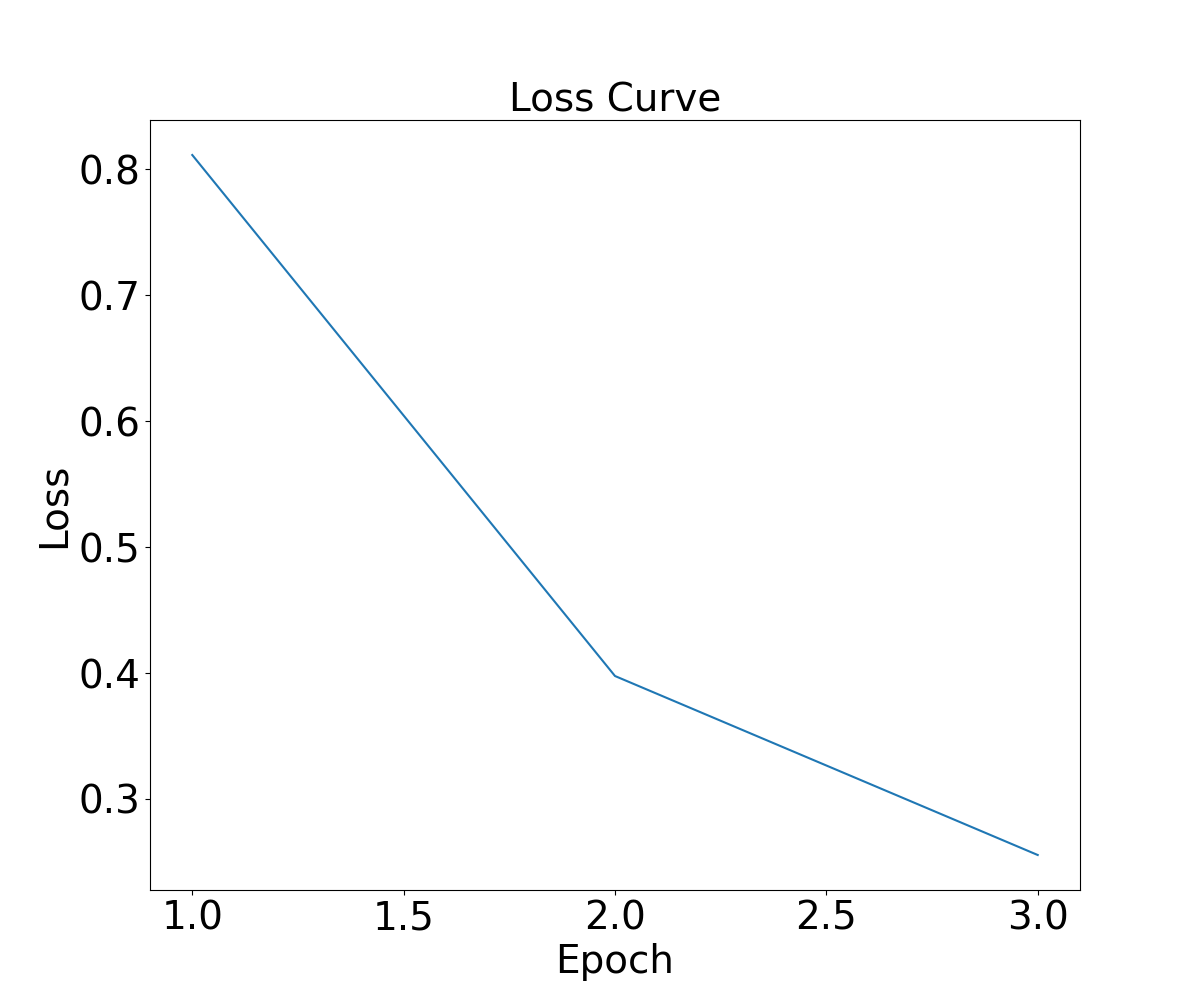
\includegraphics[width=0.32\textwidth]{loss_curve_3.png}
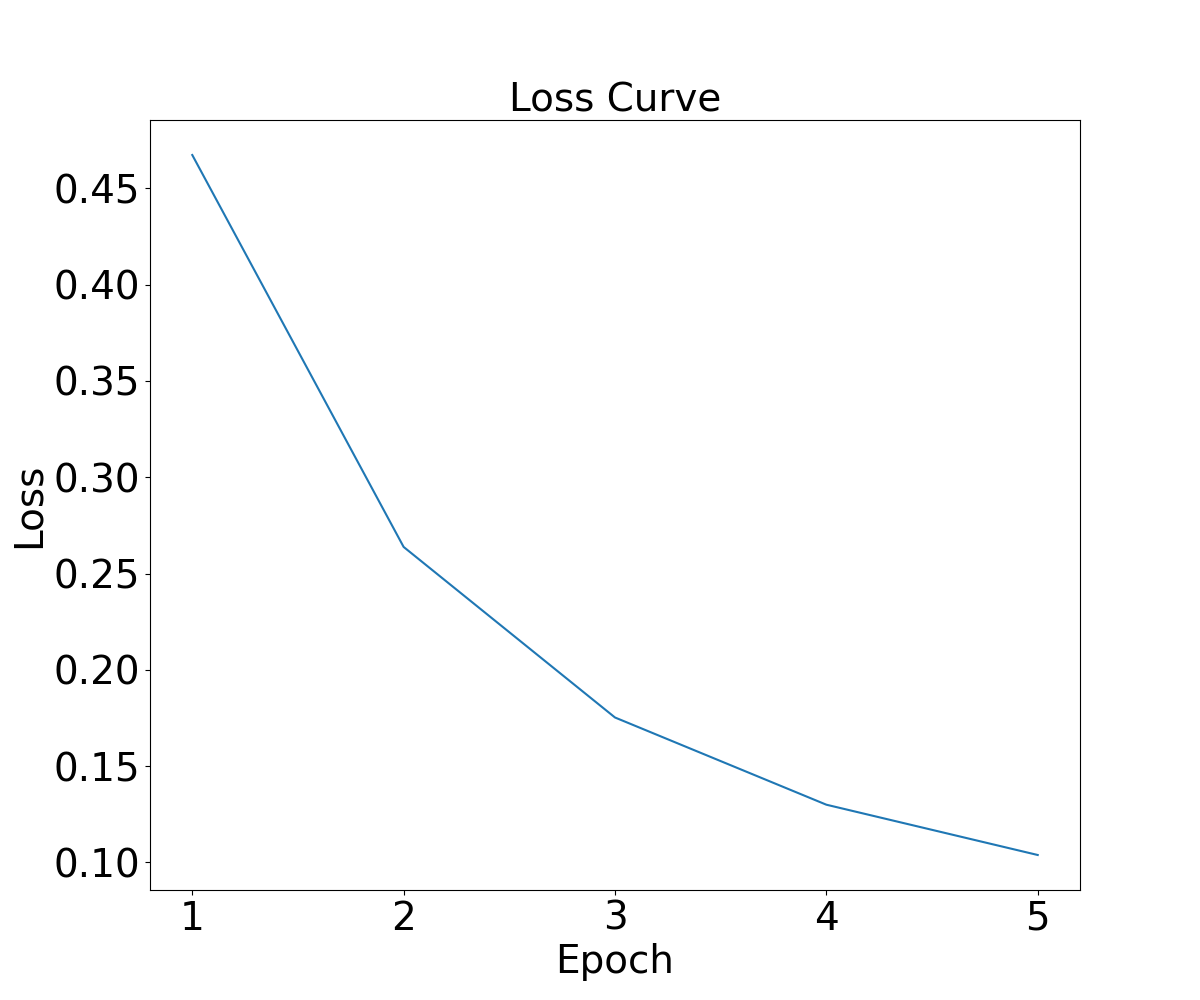
\includegraphics[width=0.32\textwidth]{loss_curve_5.png}
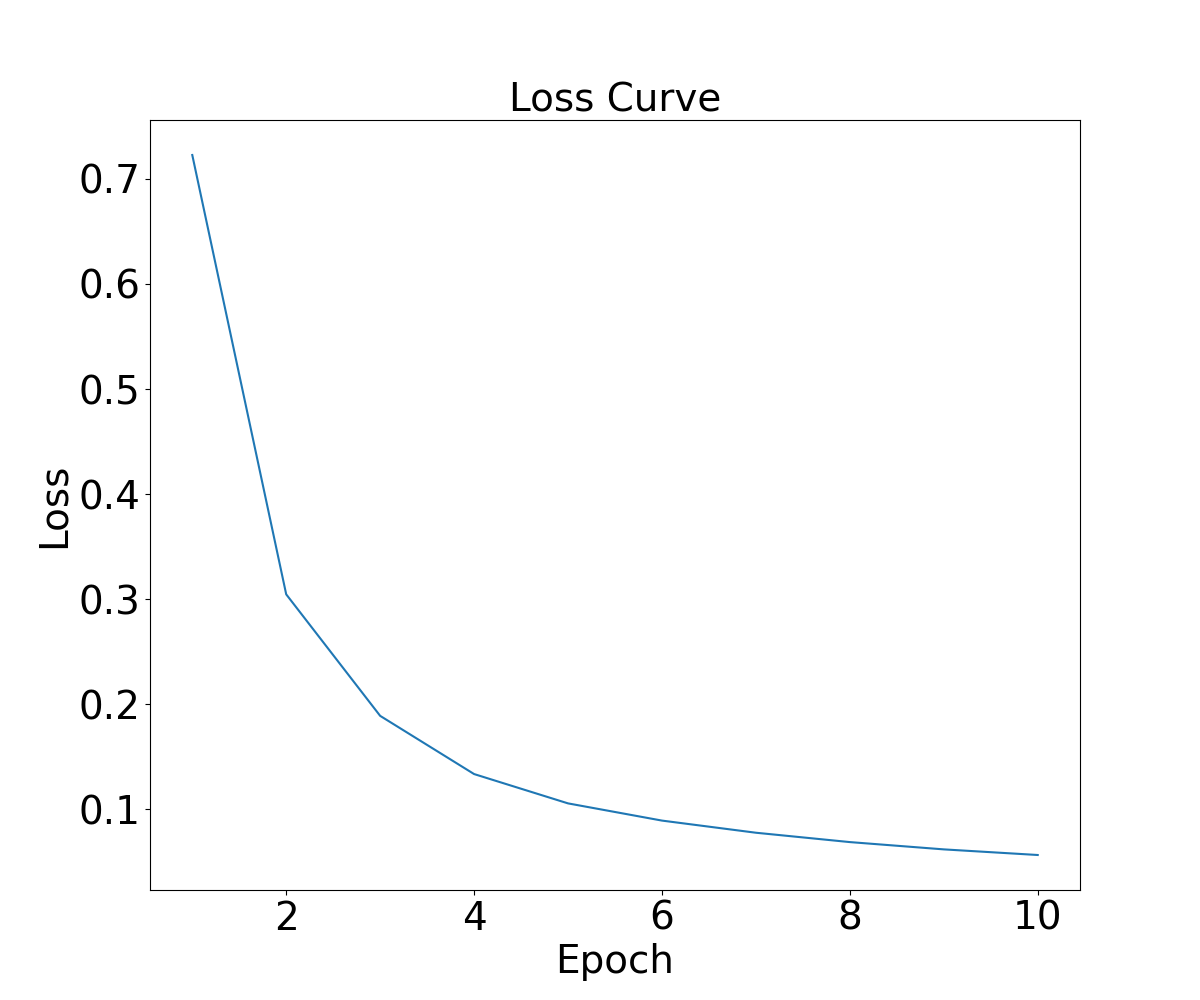
\includegraphics[width=0.32\textwidth]{loss_curve_10.png}
\caption{Loss curves over 3, 5, and 10 training epochs}
\end{figure}
\begin{figure}[H]
\centering
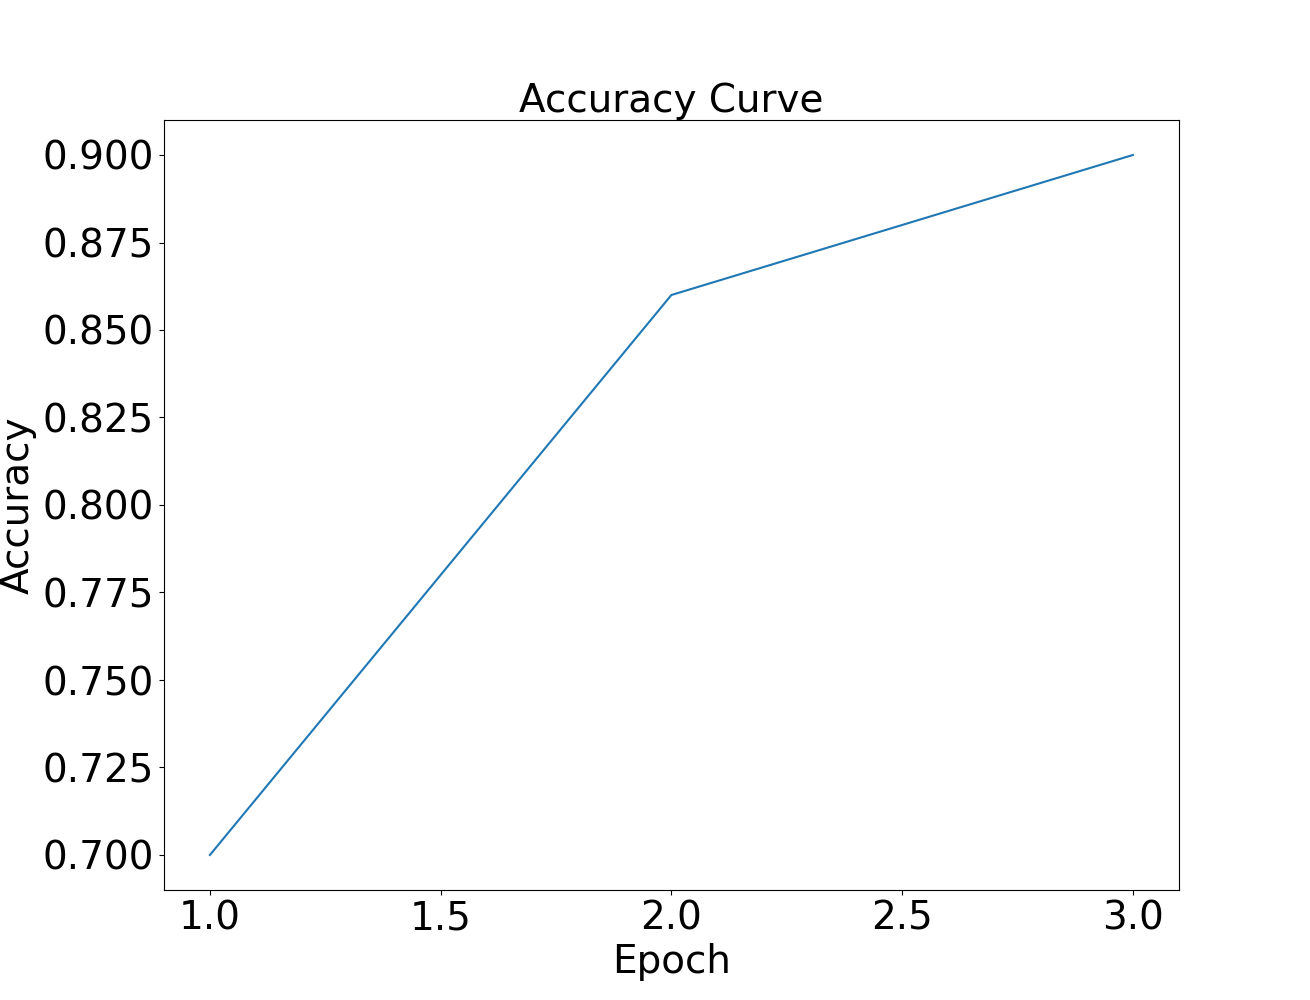
\includegraphics[width=0.32\textwidth]{accuracy_curve_3.png}
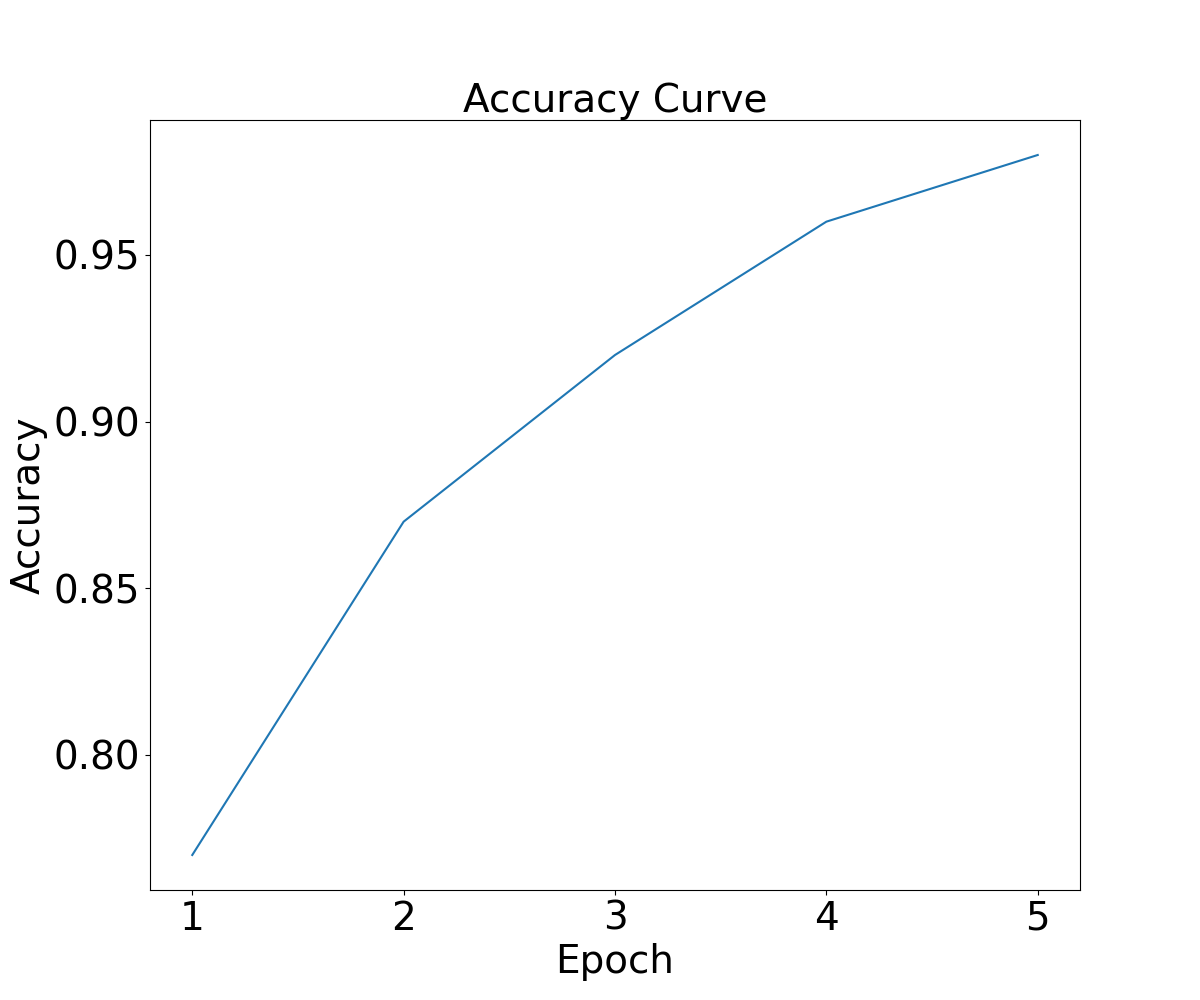
\includegraphics[width=0.32\textwidth]{accuracy_curve_5.png}
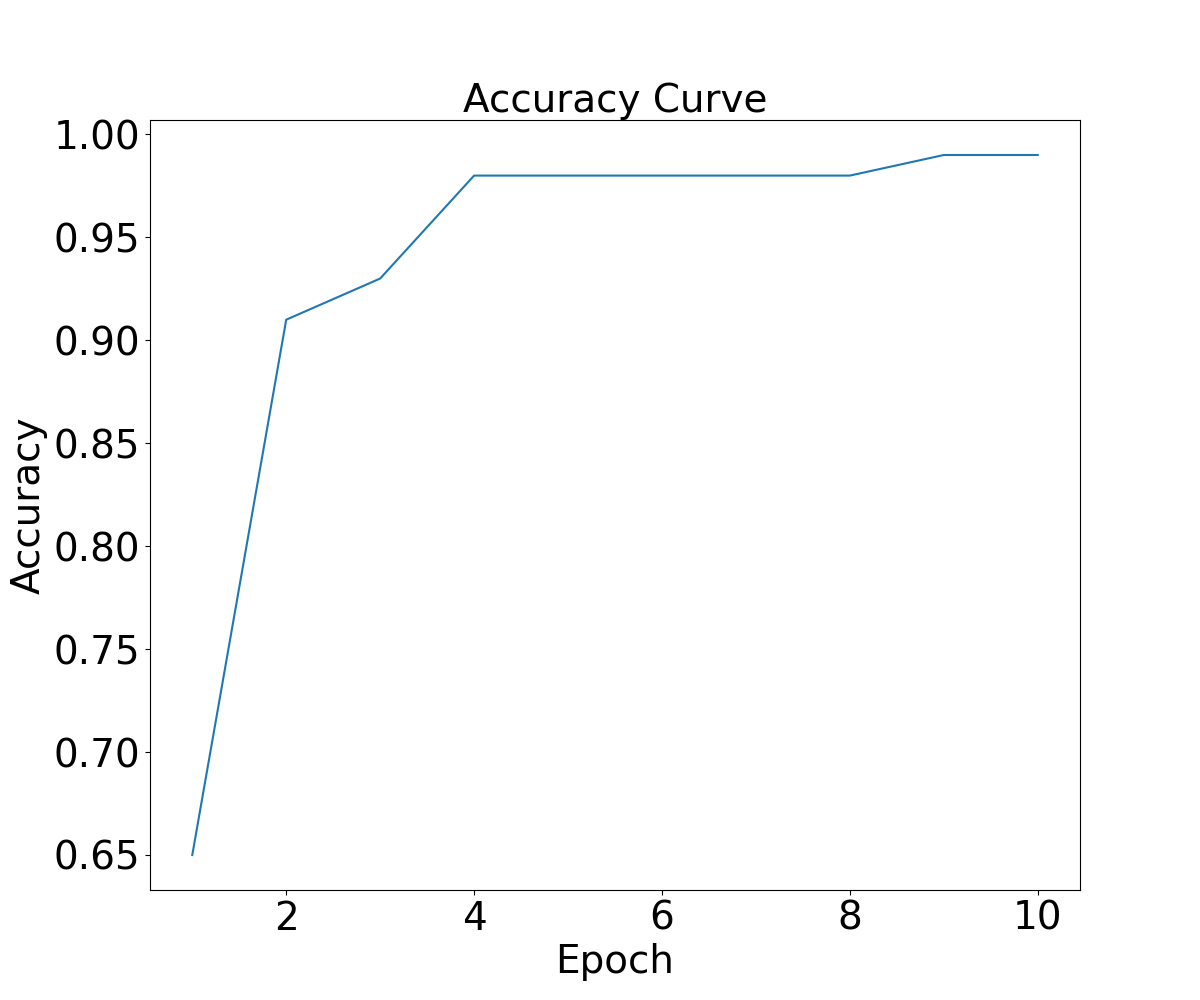
\includegraphics[width=0.32\textwidth]{accuracy_curve_10.png}
\caption{Accuracy curves over 3, 5, and 10 training epochs}
\end{figure}

Figures 1 and 2 display the loss and accuracy curves for 3, 5, and 10 training epochs. As the number of epochs increases, the loss consistently decreases, indicating improved model fitting, while the accuracy increases, reflecting better classification performance. Training for more epochs allows the network to learn more from the data, but the rate of improvement may diminish as the model approaches convergence.

\section{Discussion and Limitations}
While my pure Python implementation of a CNN offers valuable educational insights, it’s important to acknowledge its limitations and the trade-offs that come with this low-level approach. The main strength lies in its transparency—every step of the process is laid out in code, making it easy to see exactly how forward and backward passes work, how parameters are updated, and how different design choices affect the model. This kind of hands-on experience is incredibly helpful for building a deep understanding of how neural networks work under the hood.

That said, this simplicity also brings some clear limitations. The model is intentionally basic, with just one convolutional layer and one fully connected layer, which makes it unsuitable for handling more complex patterns or larger datasets. Features common in modern CNNs—like stacking multiple layers, using batch normalization, dropout, or advanced optimizers—are left out to keep things easy to follow. Plus, without automatic differentiation, all gradient calculations have to be done manually, which quickly becomes impractical as the network grows.

Performance is another challenge. Since the code doesn't take advantage of vectorized operations or GPU acceleration, even training a small network on a modest dataset can be slow. Thankfully, the MNIST dataset is clean and well-prepared, so it works well in this context and helps keep training times reasonable.

Despite these constraints, this approach is a great starting point for anyone learning about deep learning. By stripping away the complexity, it helps demystify how CNNs actually work, giving learners a stronger foundation for using high-level tools later on—and a better appreciation for the decisions that go into designing today’s deep learning frameworks.

\section{Conclusion}
In this project, I built a simple, low-level version of a convolutional neural network using only basic Python libraries. The goal was to give a clear, hands-on look at the core building blocks of deep learning—like convolution, activation functions, pooling, flattening, and dense layers. By avoiding high-level frameworks, I was able to walk through exactly how CNNs handle and learn from image data, step by step.

Even with this minimal setup, the network was able to learn meaningful patterns and perform basic classification tasks, such as telling apart digits from the MNIST dataset. Writing each part of the model by hand helped deepen my understanding of how data moves through the network, how parameters get updated, and what makes training neural networks challenging.

While this version isn’t meant for large-scale or production use, it serves as a valuable learning tool. It helps bridge the gap between theoretical knowledge and real-world implementation, giving learners a solid foundation to build on as they move to more advanced models and tools. In the future, this framework could be expanded with more layers, better optimization methods, and support for larger datasets to continue enhancing its educational impact.

\end{document}
